\documentclass[conference]{IEEEtran}
\IEEEoverridecommandlockouts
% The preceding line is only needed to identify funding in the first footnote. If that is unneeded, please comment it out.
\usepackage{cite}
\usepackage{amsmath,amssymb,amsfonts}
\usepackage{algorithmic}
\usepackage{graphicx}
\usepackage{textcomp}
\def\BibTeX{{\rm B\kern-.05em{\sc i\kern-.025em b}\kern-.08em
    T\kern-.1667em\lower.7ex\hbox{E}\kern-.125emX}}
\graphicspath{{./images/}}
\begin{document}

\title{Estimating Baseline Travel Times for the UK Strategic Road Network
%\thanks{Thanks to EPSRC and Thales UK.}
}

\author{\IEEEauthorblockN{Alvaro Cabrejas Egea}
\IEEEauthorblockA{\textit{MathSys Centre for Doctoral Training} \\
\textit{University of Warwick}\\
Coventry, United Kingdom \\
a.cabrejas-egea@warwick.ac.uk}
\and
\IEEEauthorblockN{Peter de Ford}
\IEEEauthorblockA{\textit{McKinsey \& Company} \\
	San Jose, Costa Rica \\
	pdeford@outlook.com}
\and
\IEEEauthorblockN{Colm Connaughton}
\IEEEauthorblockA{\textit{Warwick Mathematics Institute} \\
\textit{\& Centre for Complexity Science} \\
\textit{University of Warwick}\\
Coventry, United Kingdom \\
c.p.connaughton@warwick.ac.uk}
}

\maketitle

\begin{abstract}
We present a new method for estimating how the expected travel time for links on the UK Strategic Road Network varies with time.  
The approach is based on a time series analysis of travel time data from the UK's National Traffic Information Service (NTIS).  
Time series of travel times are characterised by a noisy background variation exhibiting the expected daily and weekly patterns punctuated by large spikes associated with congestion events. 
Some of these spikes are caused by peak hour congestion and some are caused by unforeseen events like accidents. 
Our algorithm uses thresholding to split the time series into background and spike signals, each of which is analysed separately. 
The daily and weekly periodic variation of the background signal is extracted using spectral filtering. 
The periodic part of the spike signal is extracted using the Seasonal-Trend Decomposition based on LOESS (STL) algorithm. 
The final estimated travel time is obtained by recombining these two. 
We assess our method by cross-validation for several UK motorways. 
We use 6 weeks of training data and calculate the mean absolute percentage error of the resulting travel time estimates for 3 subsequent weeks of test data. 
We find that the relative error is significantly reduced compared to estimates obtained by simple segmentation of the data and compared to the estimates published by the NTIS system.
\end{abstract}

\begin{IEEEkeywords}
Traffic, Congestion, Intelligent Algorithms
\end{IEEEkeywords}

\section{Introduction}
Investment in the infrastructure of transport systems is an essential driver for the economy \cite{government}. 
In developed countries such as the UK, there is limited capability to increase the physical capacity of the transport infrastructure. 
This is specifically the case for the Strategic Road Network, comprising approximately 4,400 miles of motorways and major trunk roads across England \cite{Strategic}. 
Current transportation policy and research is focused on Intelligent Mobility rather that the construction of new infrastructure: in the context of road transport, Intelligent Mobility aims to utilise new technologies and real-time data to improve the capacity and efficiency of existing physical infrastructure \cite{needs}.\\

The UK is considered world-leading in its ability to collect and process real-time data from its road network. 
Highways England are responsible for making this data available through the National Traffic Information Service (NTIS) \cite{NTIS}. 
Highways England collects data of the speed, flow, travel time and other data on the Strategic Road Network using sensors on the road and in vehicles. 
These are operated by Thales UK in collaboration with other partners.\\

Here, novel methods for generating profiles are investigated, such that they do not require segmentation or an underlying model, and that can be computed by only using statistical and spectral analysis of previous data.

\section{Data}
The NTIS employs a directed network model to represent the major roads in England; wherever a road encounters a diversion, a node is placed on the network and an edge is placed following the motorway.
The basic building blocks of the system are the so-called links. 
They are segments of these edges, with a length varying between 500 and over 6000 meters, representing carriageways in the edges between nodes connected by a road. 
The links on the network incorporate thousands of induction loops (sensors) at different sites, which report their measurements to a centralised system.\\

NTIS data is being used to assign a traffic profile to each link on the network. 
The profile gives the expected travel time at any time of day for the different sections of the Highway network, understood as the average time to transverse the links for the vehicles currently in it. 
These profiles use analysis of previous travel times within the same section of road to provide forecasts of expected future travel times and state of traffic.\\

Operating modern Smart Motorways in the UK revolves around the use of these traffic profiles; operators rely on them to identify deviations, take corrective actions and display accurate information on the overhead signs. 
In this scope, better profiles means more accuracy for the whole system.\\

Currently, generating these profiles makes use of a combination of an Exponentially Weighted Moving Average (EWMA) and heavy time-dependent segmentation, although the exact methodology is not public. 


\subsection{Data Selection}
\begin{itemize}
	\item Link-level data was extracted for sections of the M6, M11 and M25 motorways in England.
	\item The dataset for M6 and M11 comprises 90 days of data (07/03/2016-05/06/2016).
	\item The dataset for M25 comprises 75 days of data (07/04/2017-20/06/2017).
	\item Links with more than 10\% of missing data were discarded.
	\item Whenever missing data was detected for 10 or less minutes, it was linearly interpolated.
	\item Whenever missing data was detected for over 10 minutes, it was left as missing values.
\end{itemize}
The first two motorways were selected due to their high usage and combination of recurrent and outstanding congestion. 
The M25 was selected on the base that it is the most used Motorway in England on a daily basis, suffering from chronic congestion.
\subsection{Data Contents}
For each link on a specific date, the data consists of one entry per minute, containing:
\begin{itemize}
	\item Traffic speed
	\item Traffic flow
	\item Traffic headway.
	\item Current travel time
	\item Profile travel time 
	\item Free flow travel time
	\item Event flags for:
	\begin{itemize}
		\item Spontaneous congestion events
		\item Weather events 
		\item Other unspecified types of events.
	\end{itemize} 	
\end{itemize}

\subsection{Training and Testing Data}
In the case of the M6 and M11, the data comprises 12 complete weeks of travel time. The previous 8 weeks are used to predict the following 4. 
However, in an attempt to more closely simulate real operation, it was assumed that new measurements were received at the end of every week, allowing for an updated prediction using the new measurements in addition to the last 7 of the original 8 weeks used for training, effectively working on a rolling basis.\\
In the case of the M25, the dataset comprised 9 complete weeks. 
Hence, 6 weeks of data were used to predict the following 3 in the same manner as described in the previous paragraph.

\section{Examples of travel times} 
The most direct variable for measuring the state of traffic over a length of road is the vehicles' travel times. 
The travel time for a given segment of road is the average time that the vehicles currently in it are taking since they enter the segment until they exit it.\\

\begin{figure}[htbp]
	\centerline{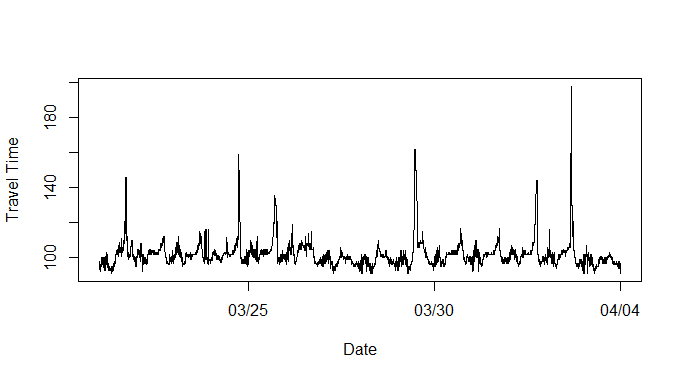
\includegraphics[width=\linewidth]{./images/Traveltime_example.png}}
	\caption{Travel times on link 117007401 in the M6 over three weeks.}
	\label{fig:travel_time_example}
\end{figure}

As it can be seen in Figure \ref{fig:travel_time_example} the travel time remains within a vaguely predictable pattern most of the days with bounded minima corresponding to the free flow time, although there are some outliers below this value corresponding to speeding drivers. 
Very low highway travel times will be found during the nights, mostly being equal to the free flow time, these will meaningfully rise as people leave to work and the add load to the motorways. 
This collective behaviour will create the morning traffic jams. 
As the morning rush passes, the travel times settle to a plateau that lasts until late afternoon when the evening rush can be observed, which potentially, albeit less likely, can also create jams. 
After this, the travel times slowly decay towards the night period of free-flow regime.\\

However, as it also follows from Figure \ref{fig:travel_time_example}, it can be seen that there are a series of excursions out of this otherwise oscillating yet bounded typical travel time. 
In these occasions the travel time can increase several times fold the usual values. These extreme oscillations are much less predictable both in intensity and inter-oscillation period than the recurrent congestion described previously.
 
\section{Current Traffic Profiles}
In this section, current approaches towards the generation of Traffic Profiles will be described, in line with how these are calculated in the United Kingdom.

\subsection{Use of Exponentially Weighted Moving Average} \label{ewma}
One currently used way for creating Traffic Profiles consists in applying an Exponentially Weighted Moving Average (EWMA) on the same minute of every day, with the implicit assumption that similar road behaviour can be expected at the same time of the day. 
Whatever changes happen for a given time, will be smooth enough so their trend will be appropriately approximated by the EWMA.
In these algorithms the Travel time forecast $F(i,d)$ on the $i-th$ minute of a given day $d$, with measured travel time $t$, will be:
\begin{equation}
F^{d+1}_i = \alpha * t^{d}_{i} + (1-\alpha)*F^{d}_{i}
\end{equation}
The main problem found when using an EWMA is the manner in which the memory decays. 
Since more recent measurements are weighted more heavily than events in the past, if an extreme fluctuation occurs in the form of a traffic jam, the following forecasts will be biased, partially replicating this event and over-estimating the travel times in that section of road until enough new measurements have been taken to dissipate this effect.

\subsection{Segmentation}\label{segmentation}
In addition, to acknowledge the specific differences between some special dates in the year, and the difference between days of the week, this family of methods requires the use of heavy date based segmentation. 
This segmentation means that the EWMA will be applied across dates which fall in the same category (i.e. Mondays, weekends, Christmas Day, ...).
If this is combined with the shortcomings presented in \ref{ewma}, it is found that some long reaching effects are generated, which can propagate for weeks into the future predictions, but do not have any reflection on the observed travel times, as it can be observed in Figure \ref{fig:EWMA_spike}.
Furthermore, in order to generate this segmentation in a valid manner, an experienced team is necessary, since the needs for segmentation can geographically vary, given that the EWMA approach tends to better approximate endemic congestion. 
This dependence on experienced teams can lead to the creation of legacy systems which may not be well understood after a few years, decreasing their usability over time unless extra effort is put into transmitting this knowledge and continually training new staff.
\begin{figure}
	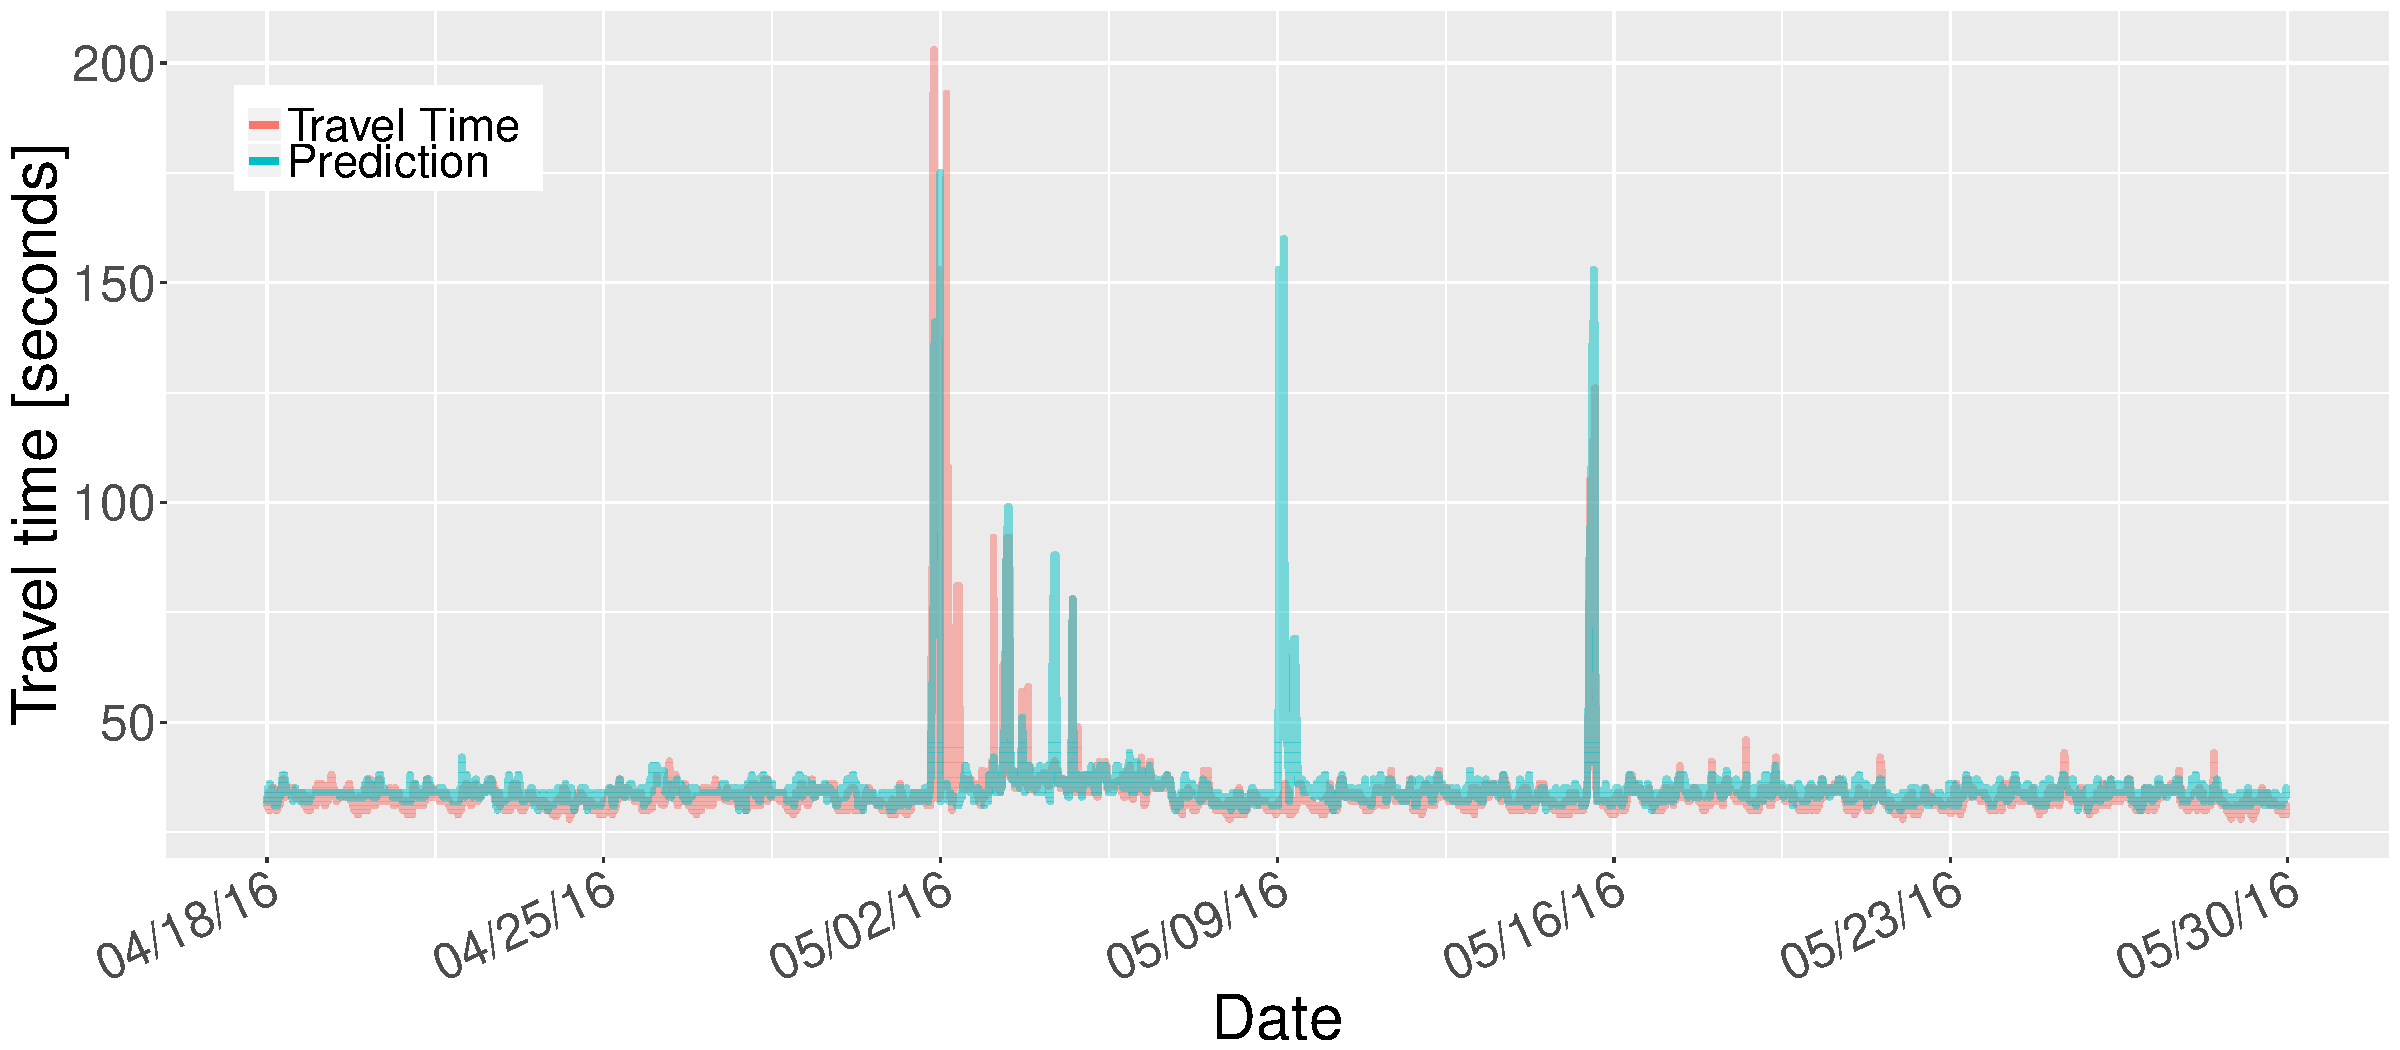
\includegraphics[width=\linewidth]{EWMA.pdf}
	\caption{Example of the current algorithm predicting increases in travel times for several weeks after a peak is seen in the measured travel times (25/04/2016)}
	\label{fig:EWMA_spike}
\end{figure}


\section{Algorithm} \label{algorithm}
Given the cyclic nature of traffic, the aim was a prediction algorithm that could account for the periodic variations and endemic congestion while being resilient to fluctuations and rare events. This algorithm also should:
\begin{itemize}
	\item Mitigate the propagation of isolated events into future forecasts.
	\item Not require the use of time segmentation (experience) and be valid for regular and "special dates".
	\item Be location agnostic, the internal parameters should be set algorithmically based on the data.
	\item Have Gaussian, mean 0, uncorrelated residuals.
	\item Near flat Trend term, given the different time scales between seasonal cycles and changes in the general motorway flow.
\end{itemize}

\subsection{Naive Segmentation}
To obtain an accurate indication of the performance of the algorithm developed in the following subsections, an example of basic segmentation was coded. 
This involved a weighted combination of the training data points using uniform weights. 
In this way, for the $i-th$ minute of a week and using a training set composed of the previous of $n$ weeks, the Naive Segmentation (NS) profile is:
\begin{equation}
NS(i,n) = \sum_{\textrm{week}=1}^{n} \frac{x^i_n}{n} 
\end{equation}

\subsection{Decomposition in Background and Spikes}
During the exploratory data analysis it was found that, from the point of view of travel times, traffic operates in two clearly differentiated regimes. 
\begin{itemize}
	\item Background: 
	\begin{itemize}
		\item Stable around a mean value.
		\item Oscillates with small amplitude and high frequency.
		\item Suitable for spectral filtering.
	\end{itemize}
	\item Spikes: 
	\begin{itemize}
		\item Zero most of the time. Quickly go to extreme values.
		\item Oscillates with great amplitude and low inter-oscillation frequency.
		\item Suitable for seasonal decomposition.
	\end{itemize}
\end{itemize}

\begin{figure}[htbp]
	\centering
	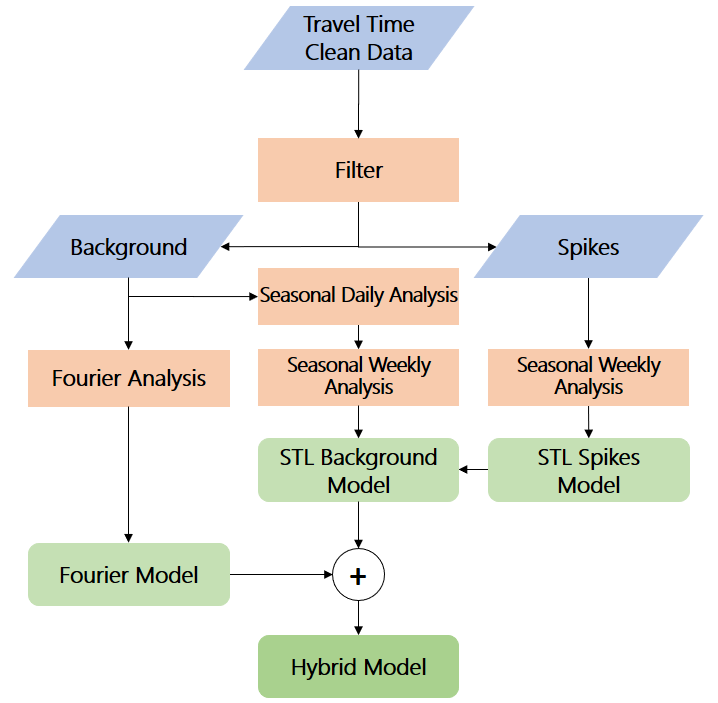
\includegraphics[width=\linewidth]{new_flow.png}
	\caption{Schematic of data streams in the algorithm.}
	\label{fig:flowchart}
\end{figure}

In order to stop the large deviations from affecting the underlying true profile, it was decided to separate these spikes from the rest and treat them in a separate manner. 
Assuming Gaussian noise $\xi$:
\begin{equation}
Travel \textrm{ } Time_t = Background_t + Spikes_t + \xi
\end{equation}
The objective was to separate them in such a way that most of the recurring congestion is captured as part of the Background and used for spectral analysis, attempting to mitigate the prediction error induced by the high frequency oscillations and obtaining a basic view of what can be daily observed.
Meanwhile, the spikes, including the recurring component not captured in the background and the non-recurring congestion, were treated separately in an attempt to find seasonality in larger time scales than those in which the background oscillates. 
Ideally, after this step, an operator should only find isolated large rare events deviating from the profile and white noise.\\

To prevent the differing lengths of the links from affecting this decomposition, for this step, all travel times were normalized according to their corresponding link's free flow time, understood as the time to transverse the length of the link at the maximum legal speed allowed by the motorway. 
However, this step only mitigates the non-regularity of the time series, since there are drivers who do not follow these limits.\\

A threshold was heuristically chosen to separate the two components in the different regimes from the normalised travel times. 
Intuitively, this threshold scales with the amount of recurring congestion in a link. 
Whenever a data point is above the threshold, it is flagged as belonging to a spike.

\begin{figure}[htbp]
	\centering
	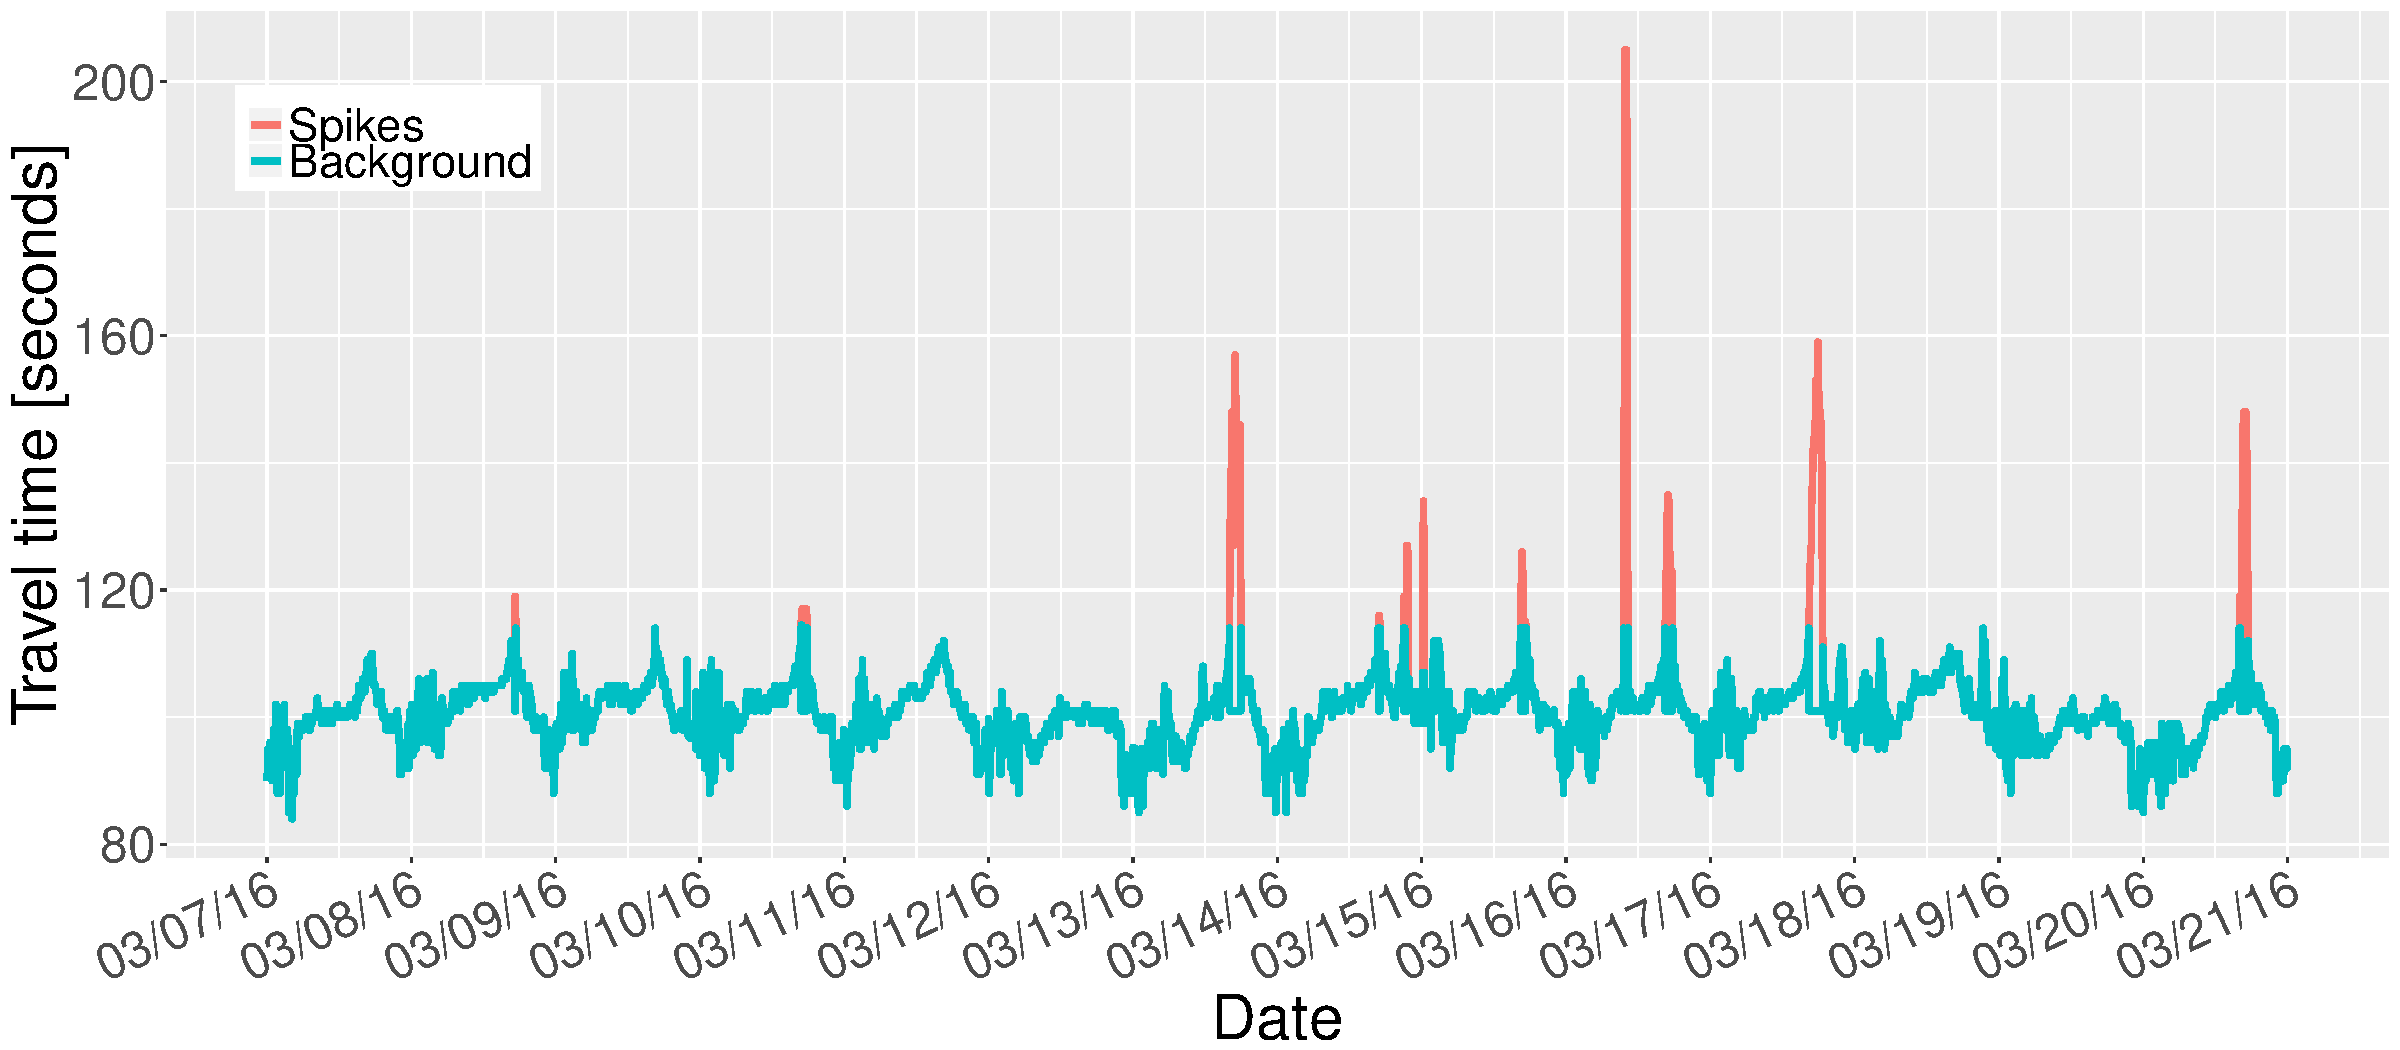
\includegraphics[width=\linewidth]{BS.pdf}
	\caption{ Decomposition of time series in background and spikes }
	\label{fig:Background}
\end{figure}

For this purpose, an indicator function was defined, taking for every minute the value:\\
\begin{equation}
\delta_t^{spike}= \left\{
\begin{array}{lr}
1 & : \textrm{Over threshold}\\
0 & : \,\,\,\,\,\,\,\,\,\,\,\,\textrm{Otherwise}
\end{array}
\right.
\label{eq:delta}
\end{equation}

\begin{table}[htbp]
	\caption{Normalised Travel Time Thresholds}
	\begin{center}
		\begin{tabular}{|c|c|}
			\hline
			\textbf{Motorway}&{\textbf{Threshold}} \\
			\hline
			M6& 1.1\\
			\hline
			M11& 1.2\\
			\hline
			M25& 1.4\\
			\hline
		\end{tabular}
		\label{tab1}
	\end{center}
\end{table}

\subsection{Spectral Component}
The main difficulty when dealing with the Background time series is the low amplitude, high frequency fluctuations that can be found almost ubiquitously. 
In these situations signal smoothing can be easily performed by removing completely the frequency components from a certain frequency and up while the information bearing low frequency components are retained. For this task, the Fast Fourier Transform (FFT) \cite{FFT} was used.

Below, the sequence of steps taken to process the Background part of the measured travel times is described
\begin{enumerate}

	\item Calculate Background Power Spectrum using FFT
	\item Remove frequencies corresponding to periods under 4 hours and over 1 week
	\item Repeat for all $n$ weeks in training set
    \item Apply and EWMA to the weekly predictions
	\item Compute the Inverse Transform

\end{enumerate}
\subsection{Seasonality Component}
Seasonal-Trend Decomposition based on LOESS (STL) \cite{STL} was chosen for the seasonality analysis since "STL has several advantages over the classical decomposition method and X-12-ARIMA: Unlike X-12-ARIMA, STL will handle any type of seasonality, not only monthly and quarterly data. 
The seasonal component is allowed to change over time, and the rate of change can be controlled by the user. 
The smoothness of the trend-cycle can also be controlled by the user. It can be robust to outliers (i.e., the user can specify a robust decomposition). 
So occasional unusual observations will not affect the estimates of the trend-cycle and seasonal components" \cite{forecasting}.\\

Below, the sequence of steps taken to process the Seasonality Component part of the measured travel times is described. 
Note that this should be applied to the $n$ training weeks as a single time series.
\begin{enumerate}
	\item STL Decomposition of Background for daily seasonality
	\item Extract and sum the series corresponding Trend and Remainder from Step 1
	\item STL decomposition for weekly seasonality
	\item Comprobation of Background's Remainder and Trend from Step 3
	\begin{enumerate}
		\item Background's Remainder should be zero mean, Gaussian distributed
		\item Background's Trend should have a near zero slope
	\end{enumerate}
	\item Add daily and weekly Seasonal components from Step 1 and Step 3 to obtain global seasonality
	\item Average seasonality across training weeks
	\item Linearise Trend term from
	\begin{enumerate}
		\item Select extreme values in the series and create a linear interpolation between them
		\item Extract the trend corresponding to the number of weeks for forecasting
	\end{enumerate}
	\item Add linearised trend to seasonality obtained in Step 6
	\item STL Decomposition of Spikes for weekly seasonality
	\item Comprobation of Spike's remainder and trend
	\begin{enumerate}
		\item Spike's Remainder should be zero mean, Gaussian distributed
		\item Spike's Trend should have a near zero slope
	\end{enumerate}
	\item Extract Spike's Seasonality corresponding to the number of weeks for forecasting
	\item Add Spike's Seasonal component to the output of 8) to output from 9)
\end{enumerate}
\subsection{Seasonal-Spectral Hybrid Profile}
In order to create the final Seasonal-Spectral Hybrid profile, referred to as Hybrid in the following sections, one of the two forecasts generated in the previous points is taken, depending on what is the identified regime, as described in 

\begin{equation}
Hybrid = Seasonal * \delta_{spike} + Spectral * (1 - \delta_{spike})
\end{equation}
Where $\delta_{spike}$ is the indicator function defined in Equation \eqref{eq:delta}.

\section{Accuracy Results}
In this section the accuracy of the algorithm described above is compared against the Published Profiles and the NS Model. 
For each temporal point $i$, the error is quantified as the average normalised distance between the prediction and the measured travel times across all analysed links.
\begin{equation}
\textrm{Error} = \left( \sum_{\textrm{Link}=1}^{n} \frac{\|\textrm{Measurement}_i - \textrm{Prediction}_i\|}{\textrm{Measurement}_i}\right) /n 
\end{equation}
\subsection{Accuracy by Quantile}
In this subsection, the accuracy of the algorithm is compared against the Published Profiles and the Null Profile across all percentiles of travel time.
As it can be seen in Figures \ref{fig:m6q}, \ref{fig:m11q} and \ref{fig:m25q}, the profile generated by combining the Seasonal and Spectral analysis has a higher accuracy than the Published Profiles and the NS Model for all percentiles of travel time except for the most extreme values where they all perform poorly.\\
The most relevant difference occurs between percentiles $[60-95]$, where the Published Profile starts to suffer from higher inaccuracy, due to some extreme events in the shorter links. 
In all cases, the Hybrid model is the one that requires greater travel times to reach a $20\%$ error in the prediction.
\begin{figure}[htbp]
	\centerline{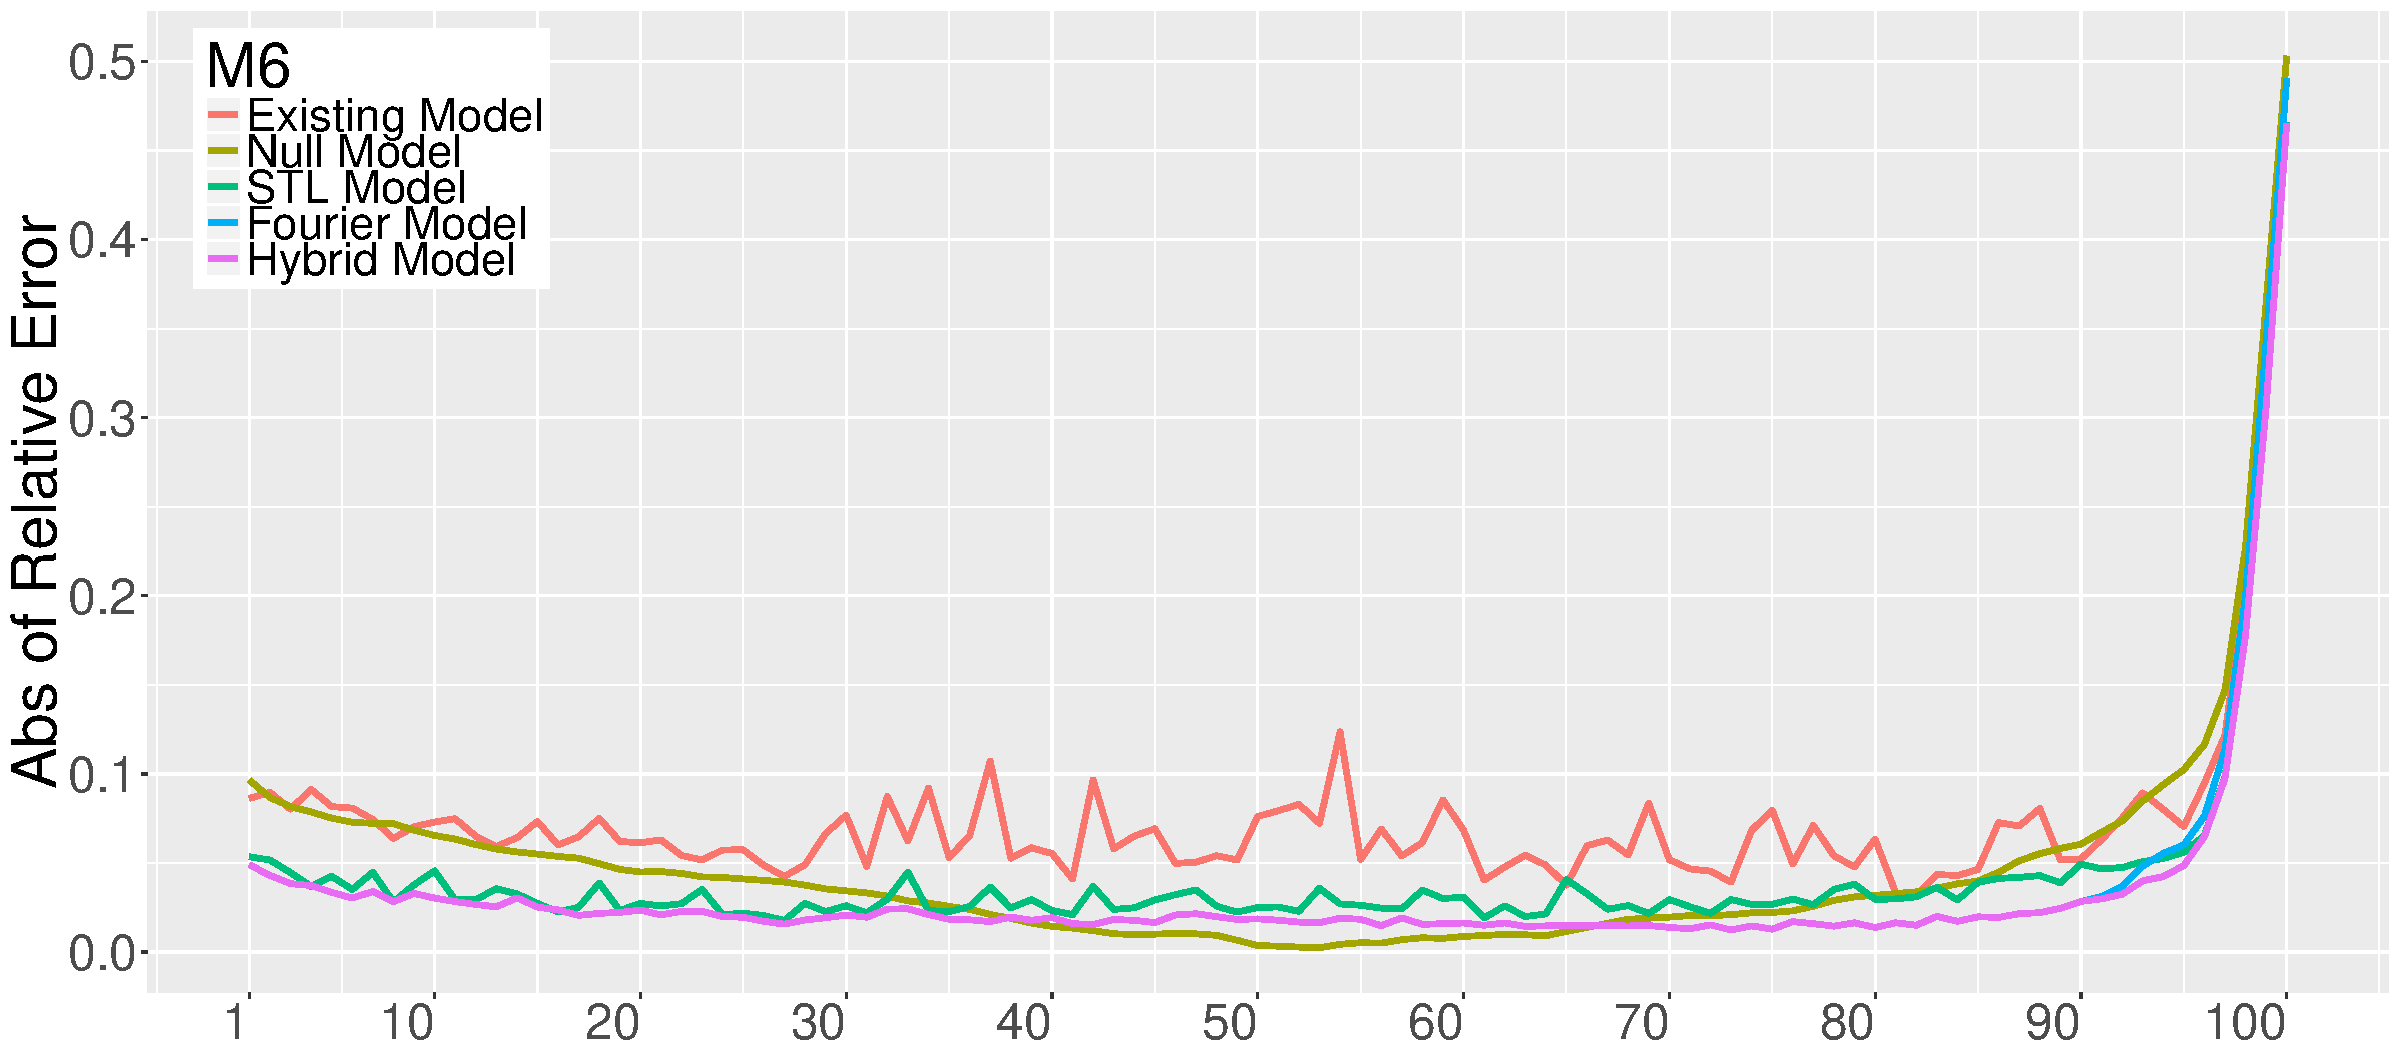
\includegraphics[width=\linewidth]{/finalplots/m6_q.pdf}}
	\caption{Average accuracy results in M6 across percentiles of travel time.}
	\label{fig:m6q}
\end{figure}

\begin{figure}[htbp]
	\centering
	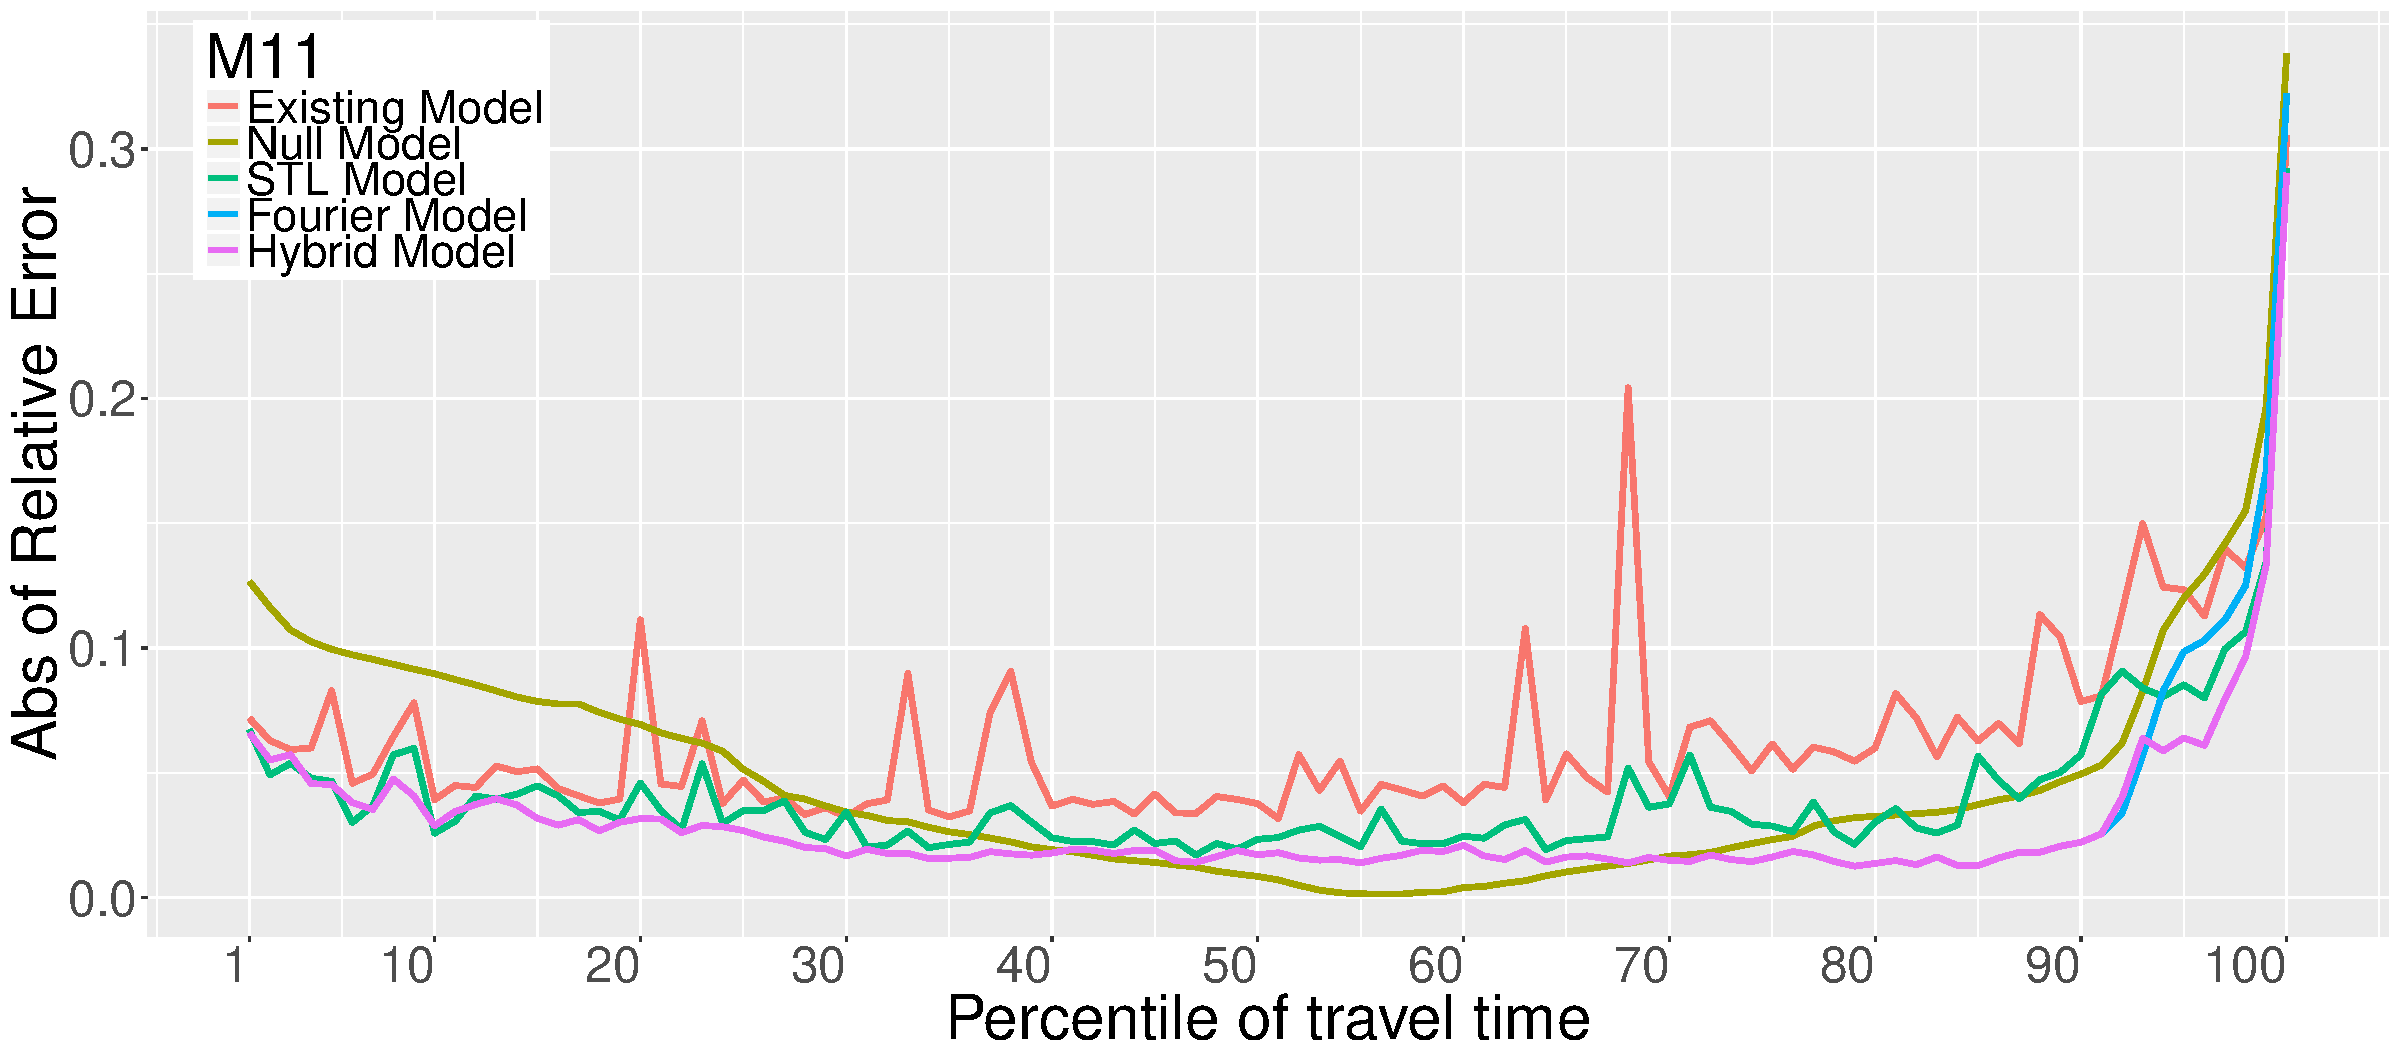
\includegraphics[width=\linewidth]{/finalplots/m11_q.pdf}
	\caption{Link average accuracy results in M11 across percentiles of travel time.}
	\label{fig:m11q}
\end{figure}

\begin{figure}[htbp]
	\centering
	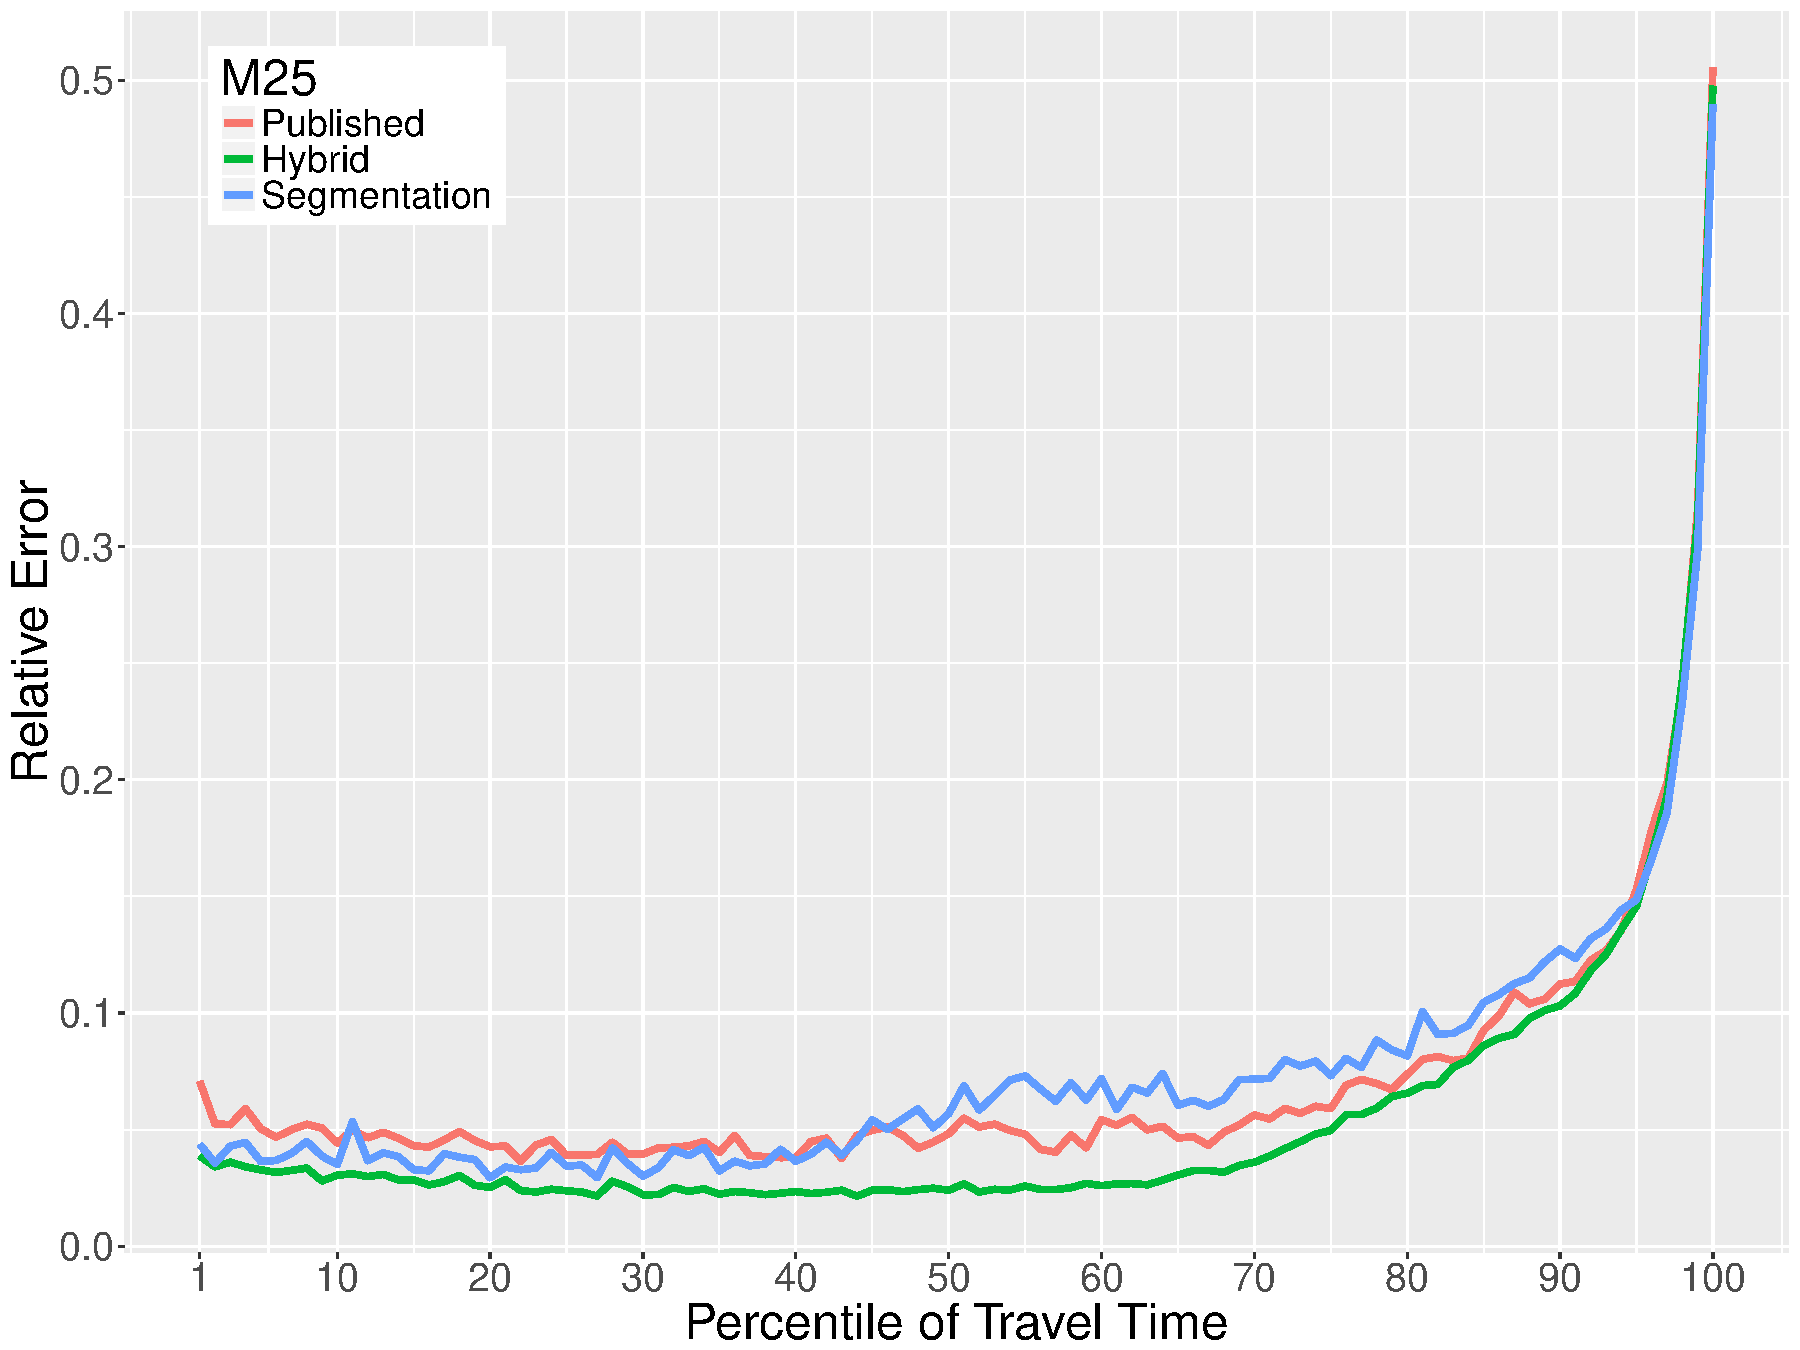
\includegraphics[width=\linewidth]{/finalplots/m25_q.pdf}
	\caption{Link average accuracy results in M25 across percentiles of travel time.}
	\label{fig:m25q}
\end{figure}

\subsection{Daytime Error}
In this subsection, the accuracy of the algorithm is compared against the Published Profiles and the Null Profile across the times of the day.
As it can be seen in Figures \ref{fig:m6daytime}, \ref{fig:m11daytime} and \ref{fig:m25daytime}, the Hybrid Profile generated by combining the Seasonal and Spectral analysis has a higher accuracy than the Published Profiles and the Null Model for all times of the day, all locations and training lengths. 
The most relevant improvement occurs during the morning and evening peak hours, where the algorithm presented in this paper does not accuse meaningful performance worsening relative to the morning plateau when compared with the other two profiles.\\
In the case of the M6 and M11, where the training set is richer, the error at peak times is reduced by at least 50\% in all cases, reaching as much as 68.7\% in the case of the M6 morning rush.
In the case of the M25, which is congested on a regular basis, the errors in the Published Profile during peak times are slightly lower than on the other cases, indicating that, given the methods used to calculate the Published Profile, this recurrent congestion is better captured by it, without the congestion being lighter in intensity than in the cases for the M6 and M11. 
Even in this case, the proposed algorithm performs significantly better than any of the other two, except for a brief window between 6-7AM when it is outperformed by the NS Model.
\begin{figure}[htbp]
	\centering
		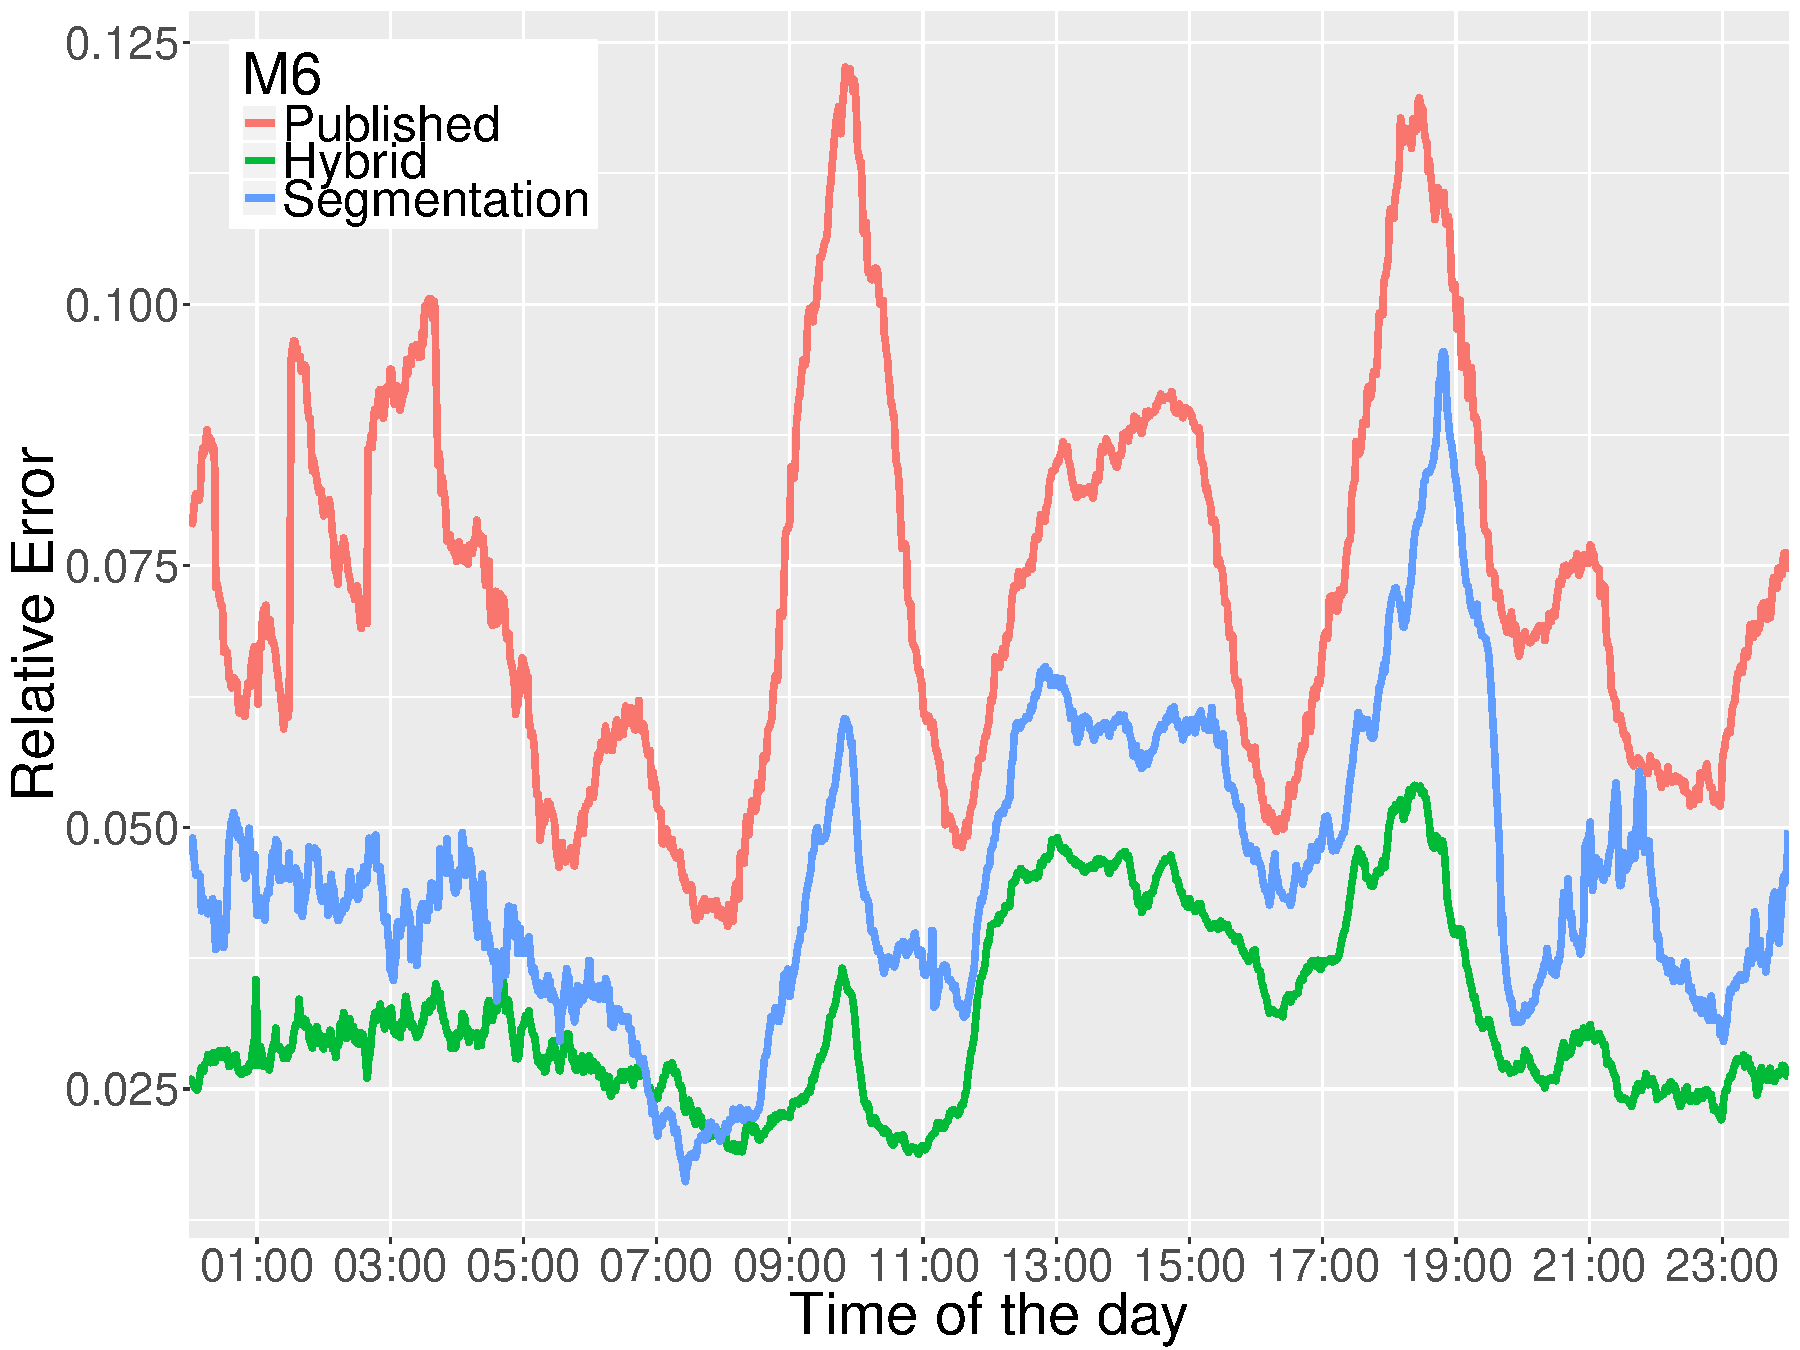
\includegraphics[width=\linewidth]{/finalplots/m6_dt.pdf}
	\caption{Link average accuracy results in M6 across times of the day.}
	\label{fig:m6daytime}
\end{figure}

\begin{figure}[htbp]
	\centering
	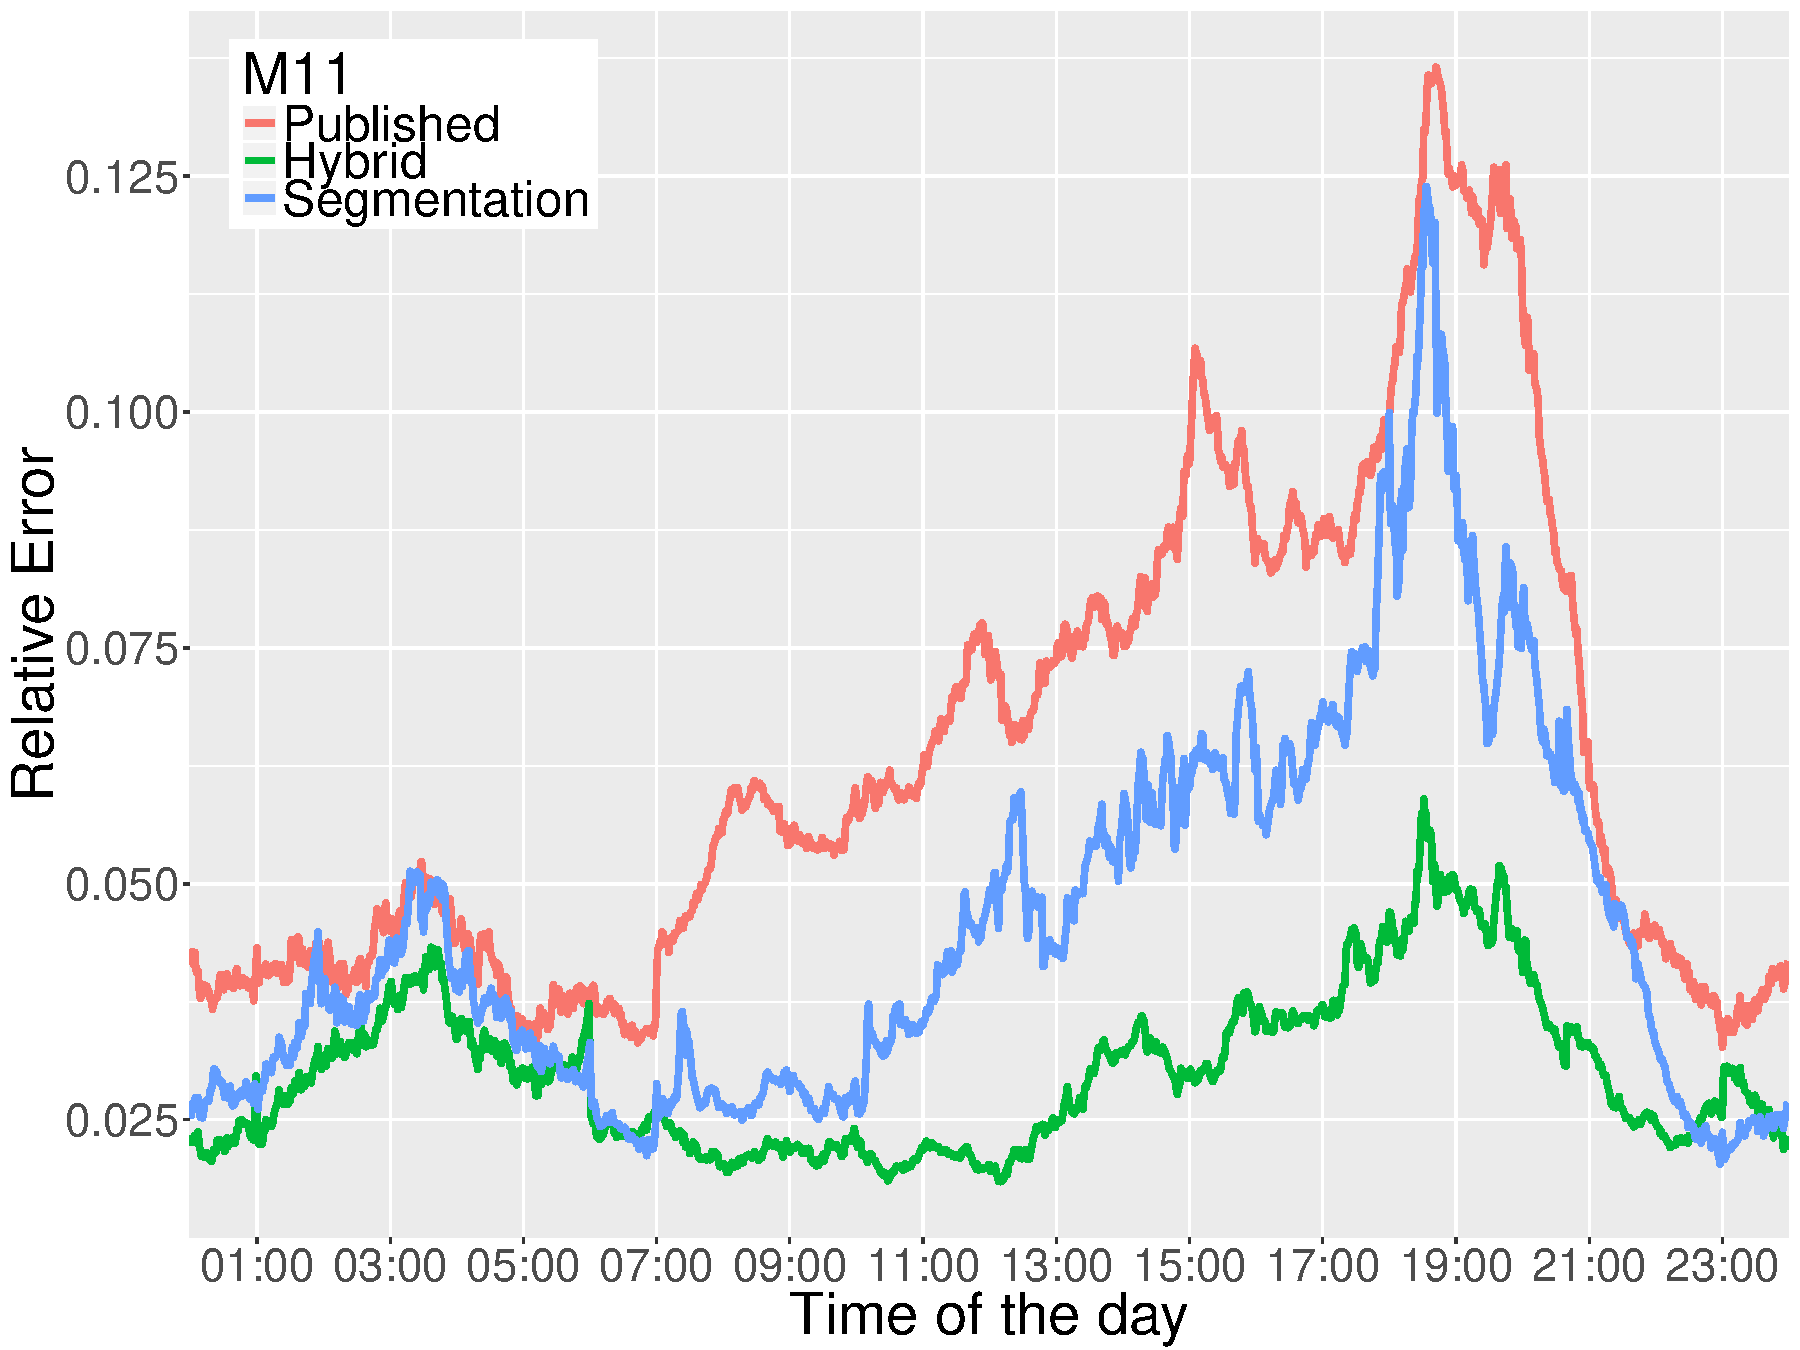
\includegraphics[width=0.95\linewidth]{/finalplots/m11_dt.pdf}
	\caption{Link average accuracy results in M6 across times of the day.}
	\label{fig:m11daytime}
\end{figure}

\begin{figure}[htbp]
	\centering
	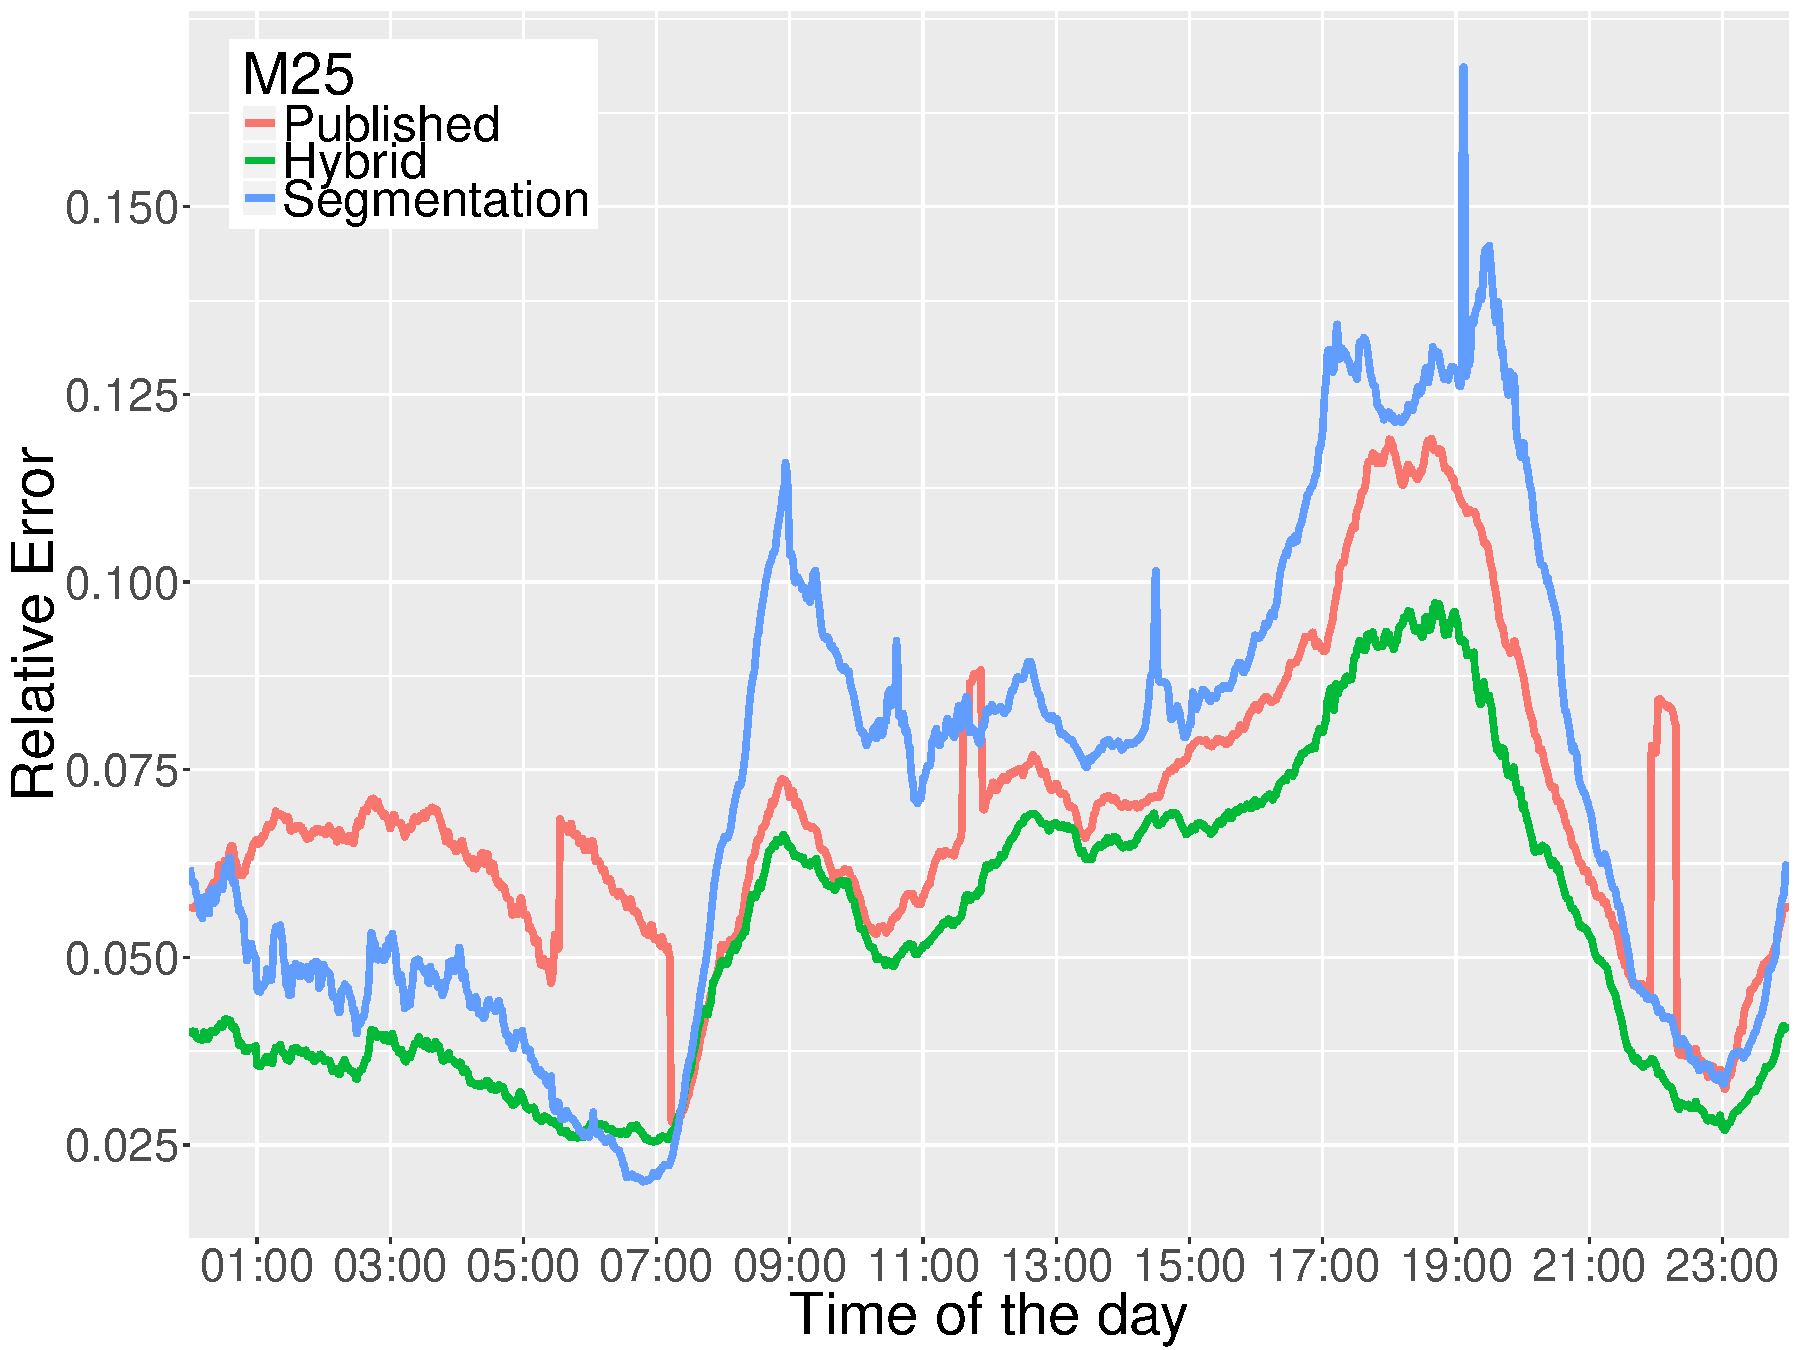
\includegraphics[width=\linewidth]{/finalplots/m25_dt.pdf}
	\caption{Link average accuracy results in M25 across times of the day.}
	\label{fig:m25daytime}
\end{figure}
\subsection{Distribution of Errors}
HERE BE MULTIPLOT(3) HISTOGRAM WITH THE DISTRIBUTION OF ERRORS, ONLY SHOW SHAPE [IGNORE?]
\section{Future Work}
The algorithm supplied above meets all the requirements described in Section \ref{algorithm} except for the fact that it requires a heuristically set threshold. 
One potential way of reaching total compliance with these requirements is to perform the decomposition between Background and Spikes by applying a Wavelet Transform. 
In the Wavelet transformed time series, it is possible to see which time scales are more affected by fluctuations and rare events while these are ongoing. 
Then, the Wavelet and Scale coefficients for those combinations of time and scale can be set to mirror those where undisturbed background can be found and the difference between these newly adapted values and the original ones would conform the Spikes series.
In the future a sensitivity analysis should be conducted to explore the limits of the algorithm in terms of minimum training data set, as well as maximum performance with increased training.
\section*{Acknowledgments}
This work was part funded by the EPSRC under grant no. EP/L015374. 
We are also grateful to the London Mathematical Laboratory for additional financial support. 
We thank Ayman Boustati, Laura Guzman Rincon and Guillem Mosquera Donate for assistance with exploratory data analysis. 
We also thank Steve Hilditch and Thales Ground Transportation Systems, UK for help understanding the NTIS system.  
A. C. E. thanks Stefan Grosskinsky for the initial guidance, discussions and support.


\begin{thebibliography}{00}
\bibitem{government} A. J. Venables, J. Laird and H. Overman, "Transport investment and economic performance: Implications for project appraisal". Technical Report, United Kingdom Department for Transport, October 2014.
\bibitem{Strategic} N. Peluffo, "Strategic road network statistics". Technical Report, United Kingdom Department for Transport, January 2015.
\bibitem{needs} P. Wockatz and P. Schartau, "Traveller needs and UK capability study", Technical Report, Transport Systems Catapult, October 2015.
\bibitem{NTIS} The Highways Agency, "National Transport Information System Publish Services", Technical Report, 2011. 
\bibitem{STL} R. B. Cleveland, W. S. Cleveland, J. E. McRae and I. Terpenning, "STL: A Seasonal-Trend Decomposition Procedure Based on Loess", Journal of Official Statistics, vol. 6, 1990, pp. 3-73.
\bibitem{forecasting} R. J. Hyndman and G. Athanasopoulos, "Forecasting: Principles and Practice", Otexts, 2013.
\bibitem{FFT} J. W. Cooley and J. W. Tukey, "An algorithm for the machine calculation of complex Fourier series", Mathematics of computation, 1965, vol. 19, no 90, p. 297-301.

\end{thebibliography}

\end{document}
